\cbox{Section word count: 1600}


First, we identified all Ecoinvent technosphere exchanges that produce waste. We then further classified the waste into non-mutually exclusive categories such as its destination (i.e., dumped, incinerated, etc.), hazardousness, and form (solid vs. liquid). After cloning the technosphere exchanges as biosphere exchanges, we aggregated and quantified them, by waste category, into matching impact categories in the Life Cycle Impact Assessment.

In our simplified test case of several battery types, we were able to identify `waste hotspots' and distinguish the major sources of contribution to waste generation on a process level. One conspicuous result from the case study (and potential direction for further work) is that many waste flows are tied to processes lacking a clear EOL pathway. Further development of this tool could involve developing an algorithm using identifiers of each background waste process to predict where these uncategorised wastes land in their EOL management.

This section is divided into two parts. In \autoref{sec:method-WMF_tool}, we describe the WasteAndMaterialFootprint tool, in \autoref{sec:method-case_study}, we describe the methodology used to calculate the waste and material footprints in the case study.

\subsection{The WasteAndMaterialFootprint tool}
\label{sec:method-WMF_tool}

The WasteAndMaterialFootprint tool is a Python package that allows one to calculate the waste and material footprint of any product or service inside of LCA databases. The tool is built on the \texttt{Brightway2} LCA framework~\citep{mutel2017brightway} and is also compatible with \texttt{ActivityBrowser}~\citep{steubing2020activitybrowser} an open-source graphical user interface for LCA. The WMF tool is installable via the Python Package Index (PyPI)~\citep{mcdowall2023wmfpipy} and is open source under the CC-0 licence. The full source code for the WasteAndMaterialFootprint tool is indexed on Zenodo~\citep{mcdowall2023wmfzenodo} and under further development in the GitHub repository~\citep{mcdowall2024wmfgithub}. The tool is designed to be used with ecoinvent databases~\citep{ecoinvent2016version3}, but could be adapted to other databases as well by changing the search criteria. Currently, it has been tested with all available system models of ecoinvent 3.5--3.10.

The program can be used directly from the command line, or imported as a Python module, in which case, the user can access the individual functions and modules. In the simplest case, the user can run the program with the default settings, which will calculate the waste and material footprint of the ecoinvent database. The user can also customise the program to calculate the waste and material footprint of a custom database, or a prospective database based on future scenarios. The program is designed to be modular so that the user can easily customise the program to their needs.

The following lists outline the constituent modules of the WMF tool, with a brief description of their functions. More extensive details can be found in the user guide and documentation of the program~\citep{mcdowall2023wmfdocs}.

\subsubsection{Functional modules:}
\begin{itemize}
    \item \texttt{future\_scenarios}: Creates prospective LCA databases based on future scenarios.
    \item \texttt{explode\_database}: Responsible for expanding a Brightway2 database into detailed exchange lists.
    \item \texttt{search\_waste}: Provides functions for searching and categorising waste generation-related exchange data.
    \item \texttt{search\_material}: Provides functions for searching and categorising material demand-related exchange data.
    \item \texttt{make\_custom\_database}: Facilitates the creation of custom databases based on the waste and material search categories.
    \item \texttt{method\_editor}: Manages the custom LCIA methods for waste and material footprint calculations.
    \item \texttt{exchange\_editor}: Appends `pseudo-biosphere' exchanges to activities to match their waste generation and material demand exchanges in the technosphere.
    \item \texttt{verify\_database}: Performs verification of the manipulated databases.
\end{itemize}

\subsubsection{Configuration modules:}
\begin{itemize}
    \item \texttt{custom\_config}: Provides functions for managing the configuration of the WasteAndMaterialFootprint package.
    \item \texttt{user\_settings}: The main configuration file, for defining the project and database settings (user editable).
    \item \texttt{queries\_waste}: Defines search parameters and categories for waste generation exchanges (user editable).
    \item \texttt{queries\_materials}: Defines search parameters and categories for material demand exchanges (user editable).
\end{itemize}

\autoref{fig:WMF_flowchart} shows the flowchart of the WasteAndMaterialFootprint tool. The subsequent subsections describe the computational framework and the modules in more detail.

\begin{figure}[h!]
    \centering
    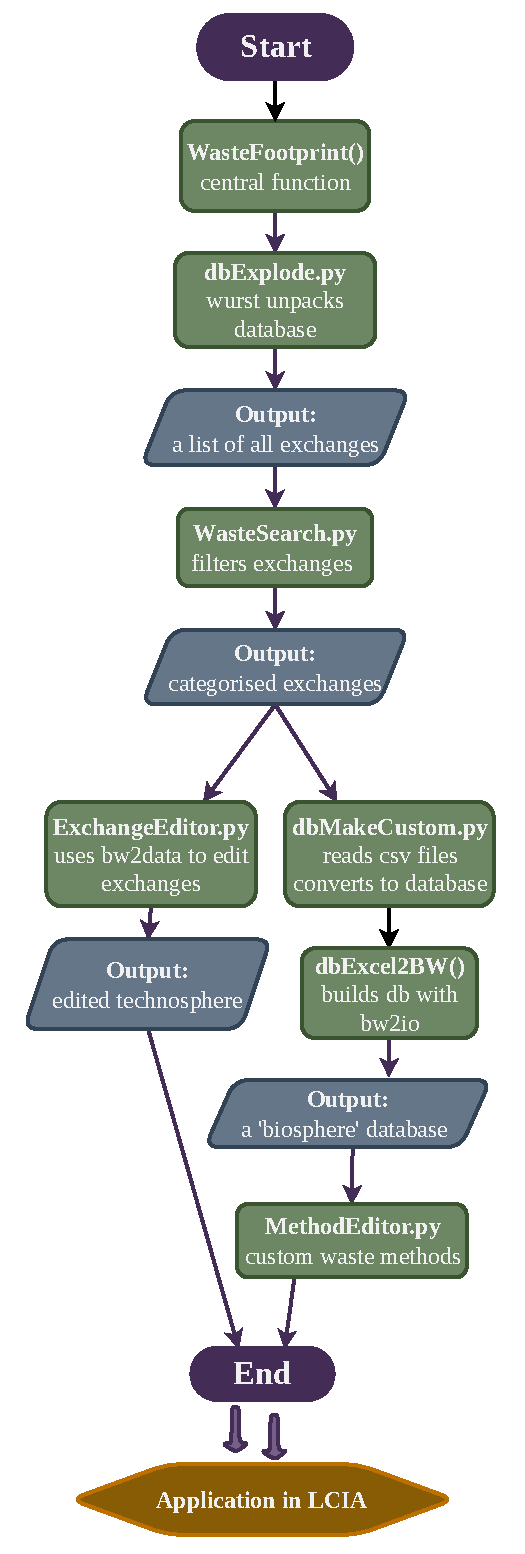
\includegraphics[width=0.7\columnwidth]{figures/WMF_flowchart.pdf}
    \caption{Flowchart of the WasteAndMaterialFootprint tool \cbox{Figure needs to be updated with new names + premise}}
    
    \label{fig:WMF_flowchart}
\end{figure}

\subsubsection{Computational framework}
Developed in the Python programming language (version 3), the WMF tool extends the brightway2 LCA framework, utilising the components \texttt{bw2data}, \texttt{bw2calc}, and \texttt{bw2io}~\citep{mutel2017brightway}. Additionally, the \texttt{wurst} package is used to facilitate database searching and data transformation at the exchange level~\citep{mutel2017wurst}. Integration with \texttt{premise} package~\citep{sacchi2022premise} enables the user to easily create and manipulate prospective LCA databases. 


\subsubsection{Generation of prospective LCA databases}
Future waste and material footprints can be projected using the \texttt{future\_scenarios} module, which uses \texttt{premise} to generate prospective scenario databases based on the configuration in \texttt{user\_settings}. These prospective databases can be custom-defined by the user or can be constructed with the future projections of the integrated assessment models such as IMAGE~\citep{stehfest2014image} and REMIND~\citep{remind2020model}, which offer a range of options aligned with the Shared Socioeconomic Pathways (SSPs)~\citep{ssp2020ghg}  that can be paired with a variety of mitigation scenarios.

\subsubsection{Database expansion}
The \texttt{explode\_database} module uses \texttt{wurst} to deconstruct LCA databases into a list of individual exchanges representing all of material and energy flows in the technosphere model. This dataset being converted into a pandas DataFrame and stored as a binary \texttt{.pickle} file for subsequent analysis.

\subsubsection{Waste and material flow identification and categorisation}

The \texttt{search\_waste} and \texttt{search\_material} modules apply user-defined search parameters from \texttt{queries\_waste} and \texttt{queries\_materials} to identify relevant waste and material flows in the list of technosphere exchanges generated by \texttt{explode\_database} and categorises them accordingly. The results of the search functions are stored in \texttt{.csv} files for subsequent use in the WMF tool's workflow.

In the default configuration, there are 10 waste categories which are further divided by their unit of measurement (kilograms and cubic meters) to create a total of 20 waste methods. The waste categories are:
\begin{itemize}[itemsep=0pt]
    \item digestion
    \item composting
    \item open burning
    \item incineration
    \item recycling
    \item landfill
    \item hazardous
    \item non-hazardous
    \item carbon dioxide (in prospective databases, carbon capture and storage is included)
    \item total
\end{itemize}

In addition to the waste categories, the \texttt{queries\_materials} module defines the material demand categories, which are based on the EU Critical Raw Materials (CRM) list for 2023~\citep{eu2023crmstudy}. The CRM list is a list of 30 materials that are considered critical to the EU economy and are at risk of supply disruption. Further materials of interest were added to the search list, including helium, electricity, petroleum, sand, water, and natural gas. The identity of the materials considered and their categorical groupings are easily customisable by the user. A full list of 59 materials included in the default configuration is provided in the supplementary material. 

\subsubsection{Creation of custom `pseudo-biosphere' databases}
Custom `pseudo-biosphere' databases are created by \texttt{make\_custom\_database} module. This module collates the waste and material categories that were present in the databases, producing an \texttt{.xlsx} file that is imported back into the Brightway2 project. 

\subsubsection{LCIA method management}
The \texttt{method\_editor} module manages the addition, deletion, and verification of the custom LCIA methods used in the WMF tool. This module uses the custom `pseudo-biosphere' databases created by \texttt{make\_custom\_database} to create these waste and material footprint LCIA methods that have the same unit as the respective technosphere exchange. The methods are stored in the Brightway2 project and can be used for calculating the waste and material footprints of activities in the LCA database in the same way as with other LCIA methods. Since `waste is not a service'~\citep{guinee2021wasteisnotaservice}, a characterisation factor of -1 is applied to the waste footprint methods, changing the perspective from waste consumed by treatment to waste generated by the activity.

\subsection{Exchange editing}
The \texttt{exchange\_editor} module loads the \texttt{.csv} files created by the search functions and appends `pseudo-biosphere' exchanges to the matching activities in the LCA database. This is the most computationally intensive part of the WMF tool, as (depending on the search configuration) there are generally more than 100,000 exchanges to be appended to the database. 

\subsubsection{Database Verification}
The \texttt{verify\_database} module calculates LCA scores for randomly selected activities using Waste Footprint and Material Demand Footprint methods to confirm that the WMF tool has processed the database correctly.

\subsection{Case Study Methodology}
\label{sec:method-case_study}

\subsubsection{Activities}
This case study investigated five types of Li-ion batteries, each represented by specific market activities:
\begin{itemize}[itemsep=0pt]
    \item Li-ion, NMC111, rechargeable, prismatic
    \item Li-ion, LiMn2O4, rechargeable, prismatic
    \item Li-ion, NCA, rechargeable, prismatic
    \item Li-ion, NMC811, rechargeable, prismatic
    \item Li-ion, LFP, rechargeable, prismatic
\end{itemize}

\subsubsection{Methods}
In addition to the Waste Footprint and Material Demand footprint methods created by the WMF tool, the following standard LCIA methods were applied for comparison:
\begin{itemize}[itemsep=0pt]
    \item ReCiPe 2016 v1.03, midpoint (I)
    \item EF v3.0 no LT
    \item EDIP 2003 no LT
    \item Crustal Scarcity
\end{itemize}

\subsubsection{Databases}
The primary source of life cycle inventory data for this case study was ecoinvent 3.9.1 cutoff. Additionally, the WMF tool was used to create prospective database sets using the \mbox{REMIND} model with the following Representative Concentration Pathways (RCPs):
\begin{itemize}
    \item \textbf{SSP2 -base:}\\ representing ca. 3.5°C increase in global temperatures to 2100
    \item \textbf{SSP2-PkBudg500:}\\ meeting Paris climate goals, ca. 1.3°C increase to 2100
\end{itemize}

For each pathway, databases were created with texttt{premise}~\citep{sacchi2022premise} and processed with the WMF tool over the time series: 2020, 2040, 2060, 2080, 2100.

\subsubsection{Calculations}
For each combination of activity, method, and database, a single score `LCIA' was calculated along with details of the top contributing processes. Additionally, for the Waste and Material Footprint methods, a contribution analysis was performed. This involved utilizing the \texttt{bwa.compare\_activities\_by\_grouped\_leaves} function from the \texttt{brightway2\_analyzer} package~\cite{mutel2016brightway2analyzer}, an additional component of the Brightway2 LCA framework. This function performs graph traversal on the impact matrix of the LCA object to a specified cutoff and groups the resulting leaves by their CPC codes. This provides insight into the products and sectors in the supply chain of the activity that carry the most responsibility for the final footprint.


